
\section{点乘(续)}\label{026}

前面比较介绍了在欧式空间里点乘的规律, 进一步地, 通过抽象化点乘这个概念,
引出了内积. 现在我们来看看两个向量的点乘到底意味着什么, 有什么用.

首先是结论: \[
\boxed{\boldsymbol{a}\cdot\boldsymbol{b}=|\boldsymbol{a}||\boldsymbol{b}|\cos\theta}.
\]

\begin{newquote}
上式中的 \(\theta\) 表示向量 \(\boldsymbol{a}\) 和 \(\boldsymbol{b}\)
之间的夹角. 等式右边的``绝对值''作用在向量上, 表示的是求向量的``大小'':
专业点说叫做``\textbf{模}'' (module); 事实上这也对应着, \(L_2\)
\textbf{范数}或者说欧氏\textbf{范数} (\(L_2\)/Euclidean norm);
理工科上也常直呼 magnitude. 很多教材也会用双竖线 \(||\cdot||\)
来标记模和范数, 用以和绝对值区分.

在三维欧式空间中, 对于
\(\boldsymbol{a}=a_x\hat{\imath}+a_y\hat{\jmath}+a_z\hat{k}\),
\(|\boldsymbol{a}|\equiv\sqrt{\boldsymbol{a}\cdot\boldsymbol{a}}=\sqrt{a_x^2+a_y^2+a_z^2}\).
\end{newquote}

上面的结论可以用余弦定律 (参见【\ref{005}\nameref{005}】) 来推导:

\begin{tcolorbox}[size=fbox, breakable, enhanced jigsaw]
  % \includegraphics[width=0.4\textwidth]{img/image-20231218163322717.png}
\end{tcolorbox}

\begin{newquote}
证明: 利用余弦定律有 \[
|\boldsymbol{a}|^2+|\boldsymbol{b}|^2-2|\boldsymbol{a}||\boldsymbol{b}|\cos\theta=|\boldsymbol{b}-\boldsymbol{a}|^2
\] 对等式右边展开有:
\(|\boldsymbol{b}-\boldsymbol{a}|^2=|\boldsymbol{a}|^2+|\boldsymbol{b}|^2-2\boldsymbol{a}\cdot\boldsymbol{b}\),
和完全平方的展开非常类似 (这一结论可以从分量的运算看出),
不过交叉项严格来说
\(-\boldsymbol{a}\cdot\boldsymbol{b}-\boldsymbol{b}\cdot\boldsymbol{a}\),
只因\footnote{只因你太美, baby.}点乘满足交换律,
于是两个交叉项事实上没有区别
(不难从【\ref{025}\nameref{025}】中发现点乘是满足交换律和结合律的). 于是 \[
|\boldsymbol{a}|^2+|\boldsymbol{b}|^2-2|\boldsymbol{a}||\boldsymbol{b}|\cos\theta=|\boldsymbol{a}|^2-|\boldsymbol{b}|^2-2\boldsymbol{a}\cdot\boldsymbol{b},
\] 遂得到结论.
\end{newquote}

这样一来, 点乘的一个应用便是找到两个向量之间的夹角. 利用这个夹角,
便可以求得一个向量在另一个向量方向上的``投影'' (projection)\footnote{``投影''其实说得很``物理'',
  考虑上文附图中, 光线沿着垂直于b的方向照在a上, 然后在b上 cast
  了一个阴影, 阴影的长度就叫a在b方向上的投影.}:

  \begin{tcolorbox}[size=fbox, breakable, enhanced jigsaw]
    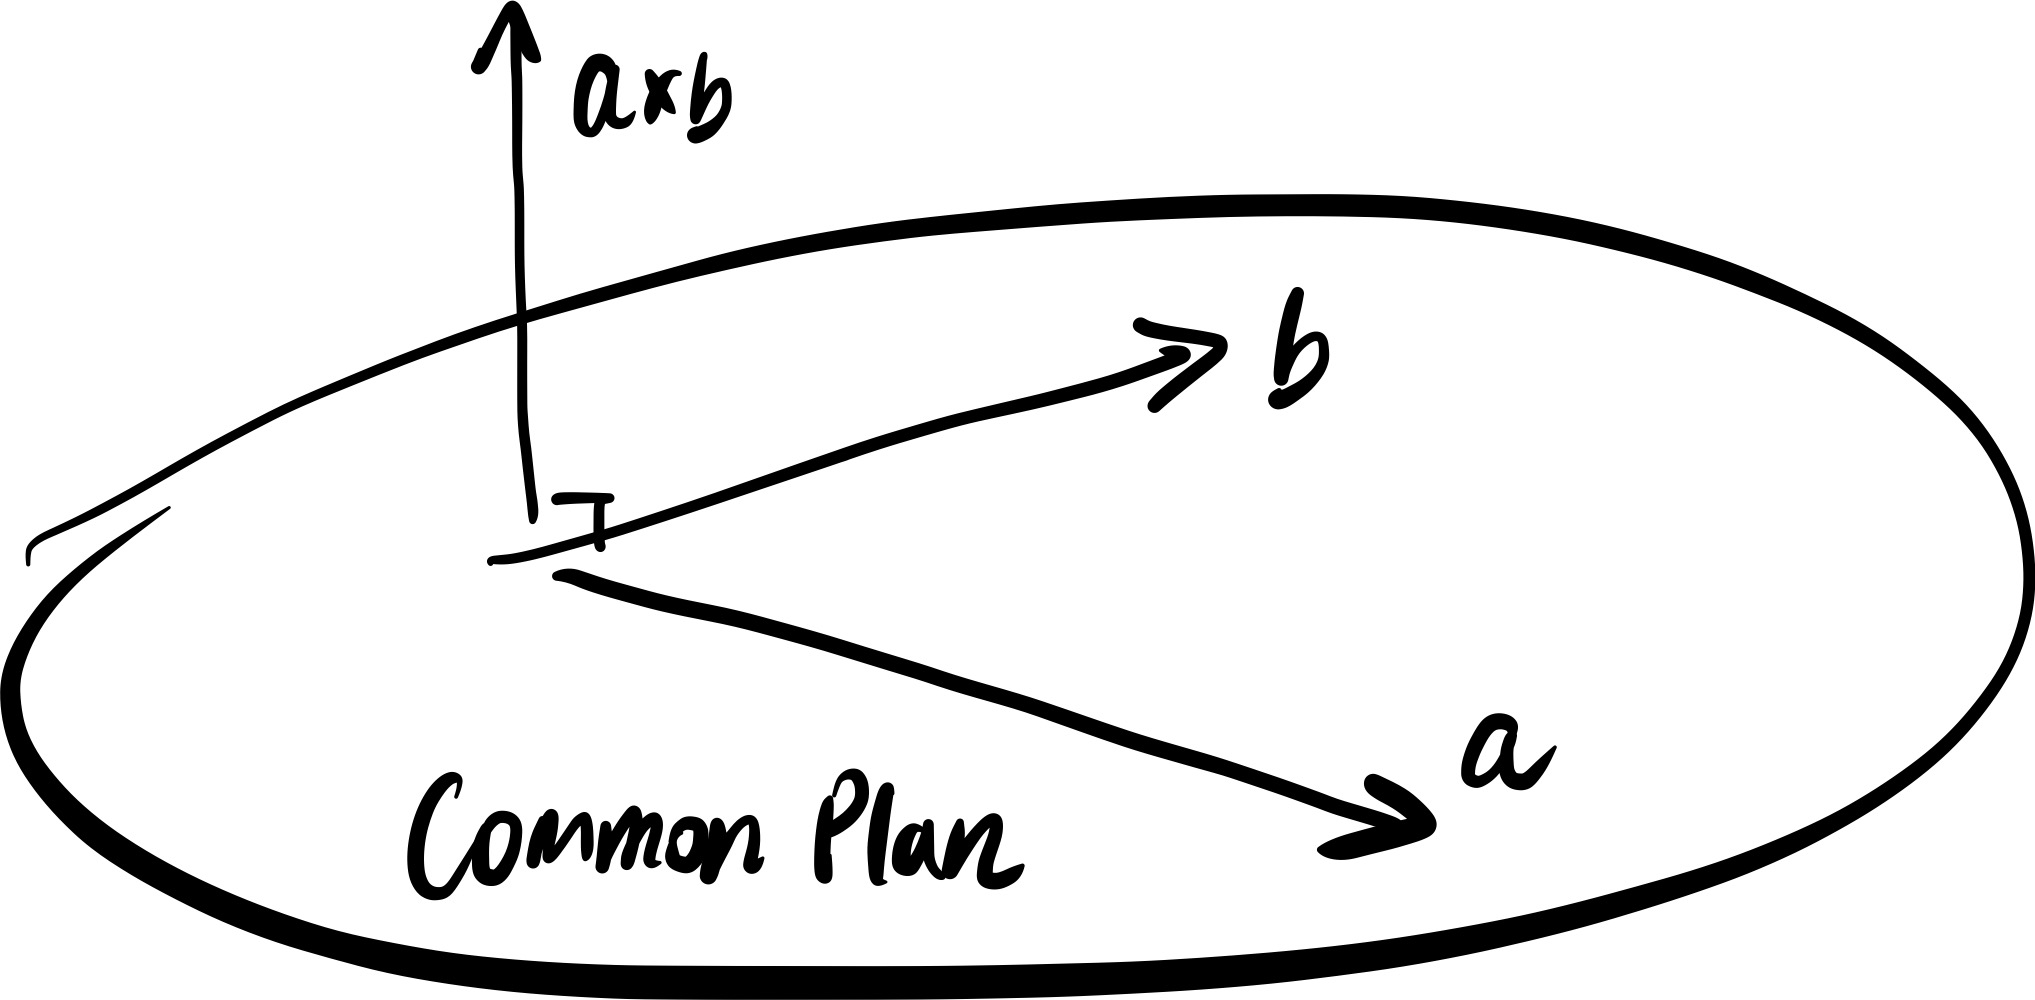
\includegraphics[width=0.4\textwidth]{img/image-20240104090927918.png}
  \end{tcolorbox}

如上图所示, \(\boldsymbol{a}\) 和 \(\boldsymbol{b}\) 的夹角 \(\theta\)
的余弦利用点乘可得是
\(\frac{\boldsymbol{a}\cdot\boldsymbol{b}}{|\boldsymbol{a}||\boldsymbol{b}|}\),
于是 \(\boldsymbol{a}\) 在 \(\boldsymbol{b}\) 方向上``投影''的长度是
\(|\boldsymbol{a}|\cos\theta=|\boldsymbol{a}|\frac{\boldsymbol{a}\cdot\boldsymbol{b}}{|\boldsymbol{a}||\boldsymbol{b}|}=\frac{\boldsymbol{a}\cdot\boldsymbol{b}}{|\boldsymbol{b}|}\),
``投影''这个向量还需要加上方向的信息, 于是有
\[
\mathrm{proj}_{\boldsymbol{b}}(\boldsymbol{a})=\frac{\boldsymbol{a}\cdot\boldsymbol{b}}{|\boldsymbol{b}|}\frac{\boldsymbol{b}}{|\boldsymbol{b}|}.
\]
很多场合下, \(\frac{\boldsymbol{b}}{|\boldsymbol{b}|}\) 这样表示向量
\(\boldsymbol{b}\) 方向上的单位向量, 经常记作 \(\hat{\boldsymbol{b}}\).


\subsubsection{叉乘}
叉乘是在三维偶氏空间 \(\mathbb{R}^3\) 中的一个特殊运算,
两个任意线性不相关的向量存在于一个公共的平面 (两条直线确定一个平面),
这样两个向量的叉乘则给出了一个垂直于这个平面的向量,
在或者说是它们共面的法向量 (normal vector) ,
再或者说同时垂直于它们二者的新的向量; 法向量的指向可以通过右手定则确定
(四指从第一个向量握向第二个向量,
拇指的指向便是这两个向量叉乘的结果的方向), 因此叉乘有反交换率,
i.e.~\(\boldsymbol{a}\times\boldsymbol{b}=-\boldsymbol{b}\times\boldsymbol{a}\).

计算上, 可以利用行列式 (determinant, 虽然还没正式介绍\ldots),
例如考虑\(\boldsymbol{a}=a_x\hat{\imath}+a_y\hat{\jmath}+a_z\hat{k}\) 和
\(\boldsymbol{b}=b_x\hat{\imath}+b_y\hat{\jmath}+b_z\hat{k}\),
它们的叉乘是 \[
\boldsymbol{a}\times\boldsymbol{b}=\begin{vmatrix}\hat{\imath}&\hat{\jmath}&\hat{k}\\a_x&a_y&a_z\\b_x&b_y&b_z\end{vmatrix},
\] 展开便是 \[
\boldsymbol{a}\times\boldsymbol{b}=(a_yb_z-a_zb_y)\hat{\imath}+(a_zb_x-a_xb_z)\hat{\jmath}+(a_xb_y-a_yb_x)\hat{k}.
\]

\begin{tcolorbox}[size=fbox, breakable, enhanced jigsaw]
  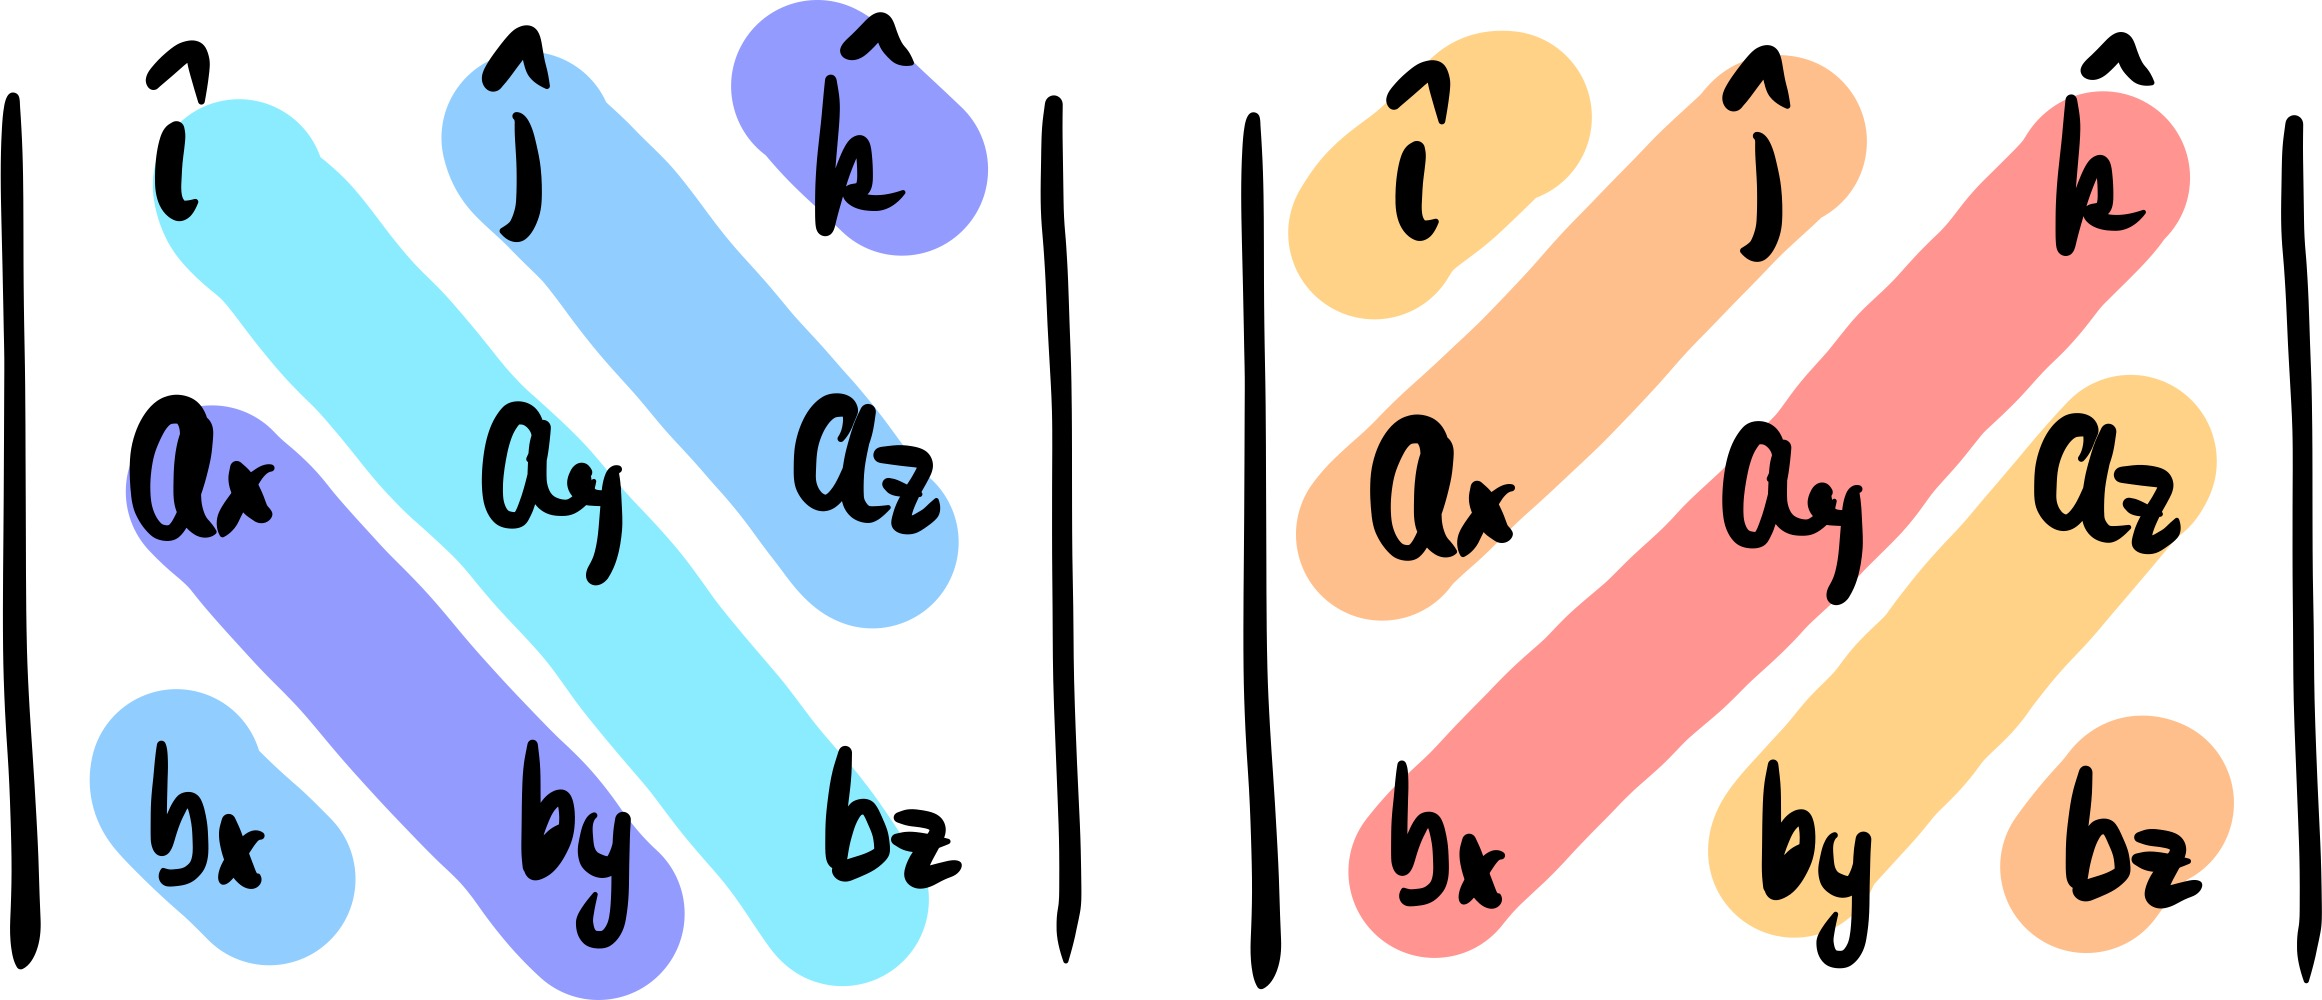
\includegraphics[width=0.4\textwidth]{img/image-20240104090600239.png}
  [size=fbox, breakable, enhanced jigsaw, sidebyside]
  \kaishu{
    个人的记忆方法是, 左上向右下的对角线之和
    (凑不够三项相乘的对称到另一边补), 减去右上向左下的对角线之和.
  }
\end{tcolorbox}

叉乘本身不能推广到更高维, 但是叉乘事实上是楔积 (wedge product)
\(\wedge\), 楔积便没有维度的限制了, 并且【\ref{021}\nameref{021}】中提到的体积元,
更严格来讲应该是类似
\(\mathrm{d}V=\mathrm{d}x\wedge\mathrm{d}y\wedge\mathrm{d}z\).

\begin{newquote}

\textbf{关于楔积, 外积, 和张量积} - 选读

楔积也叫做外积 (exterior product), 命名和``内''相对的原因: 以
\(\mathbb{R}^3\) 为例, 内积使得原来两个向量变成了一个标量,
损失了一些信息, ``缩并''\footnote{Spoiler alert: 指标缩并 (index
  contraction).}向内了;
而外积则产生了原先两个向量共面之``外''的一个向量.

【\ref{025}\nameref{025}】讨论内积的时候, 我们借用了狄拉克记号, 其中有
\(\left|\ \right>\left<\ \right|\) 这样一个操作, 因为和内积
\(\left<\ \right|\left.\right>\) 正好反过来, 于是很多时候被称为 outer
product, 并没有对应的中文 (不是外积! 不是外积! 不是外积!),
这个运算事实上是张量积.

利用行/列向量, 和矩阵乘法的规则 (左边的行乘右边的列), 考虑
$\boldsymbol{a}=\begin{pmatrix}a_x\\a_y\end{pmatrix}$,
$\boldsymbol{b}=\begin{pmatrix}b_x\\b_y\end{pmatrix}$, 内积和外积分别是

\begin{align*}
\left<{\boldsymbol{a}}\right|\left.\boldsymbol{b}\right>\Rightarrow&\boldsymbol{a}^T\boldsymbol{b}\\
=&\begin{pmatrix}a_x&a_y\end{pmatrix}\begin{pmatrix}b_x\\b_y\end{pmatrix}\\
=&a_xb_x+a_yb_y\Rightarrow\boldsymbol{a}\cdot\boldsymbol{b};
\end{align*}

\begin{align*}
\left|{\boldsymbol{a}}\right>\left<{\boldsymbol{b}}\right|\Rightarrow&\boldsymbol{a}\boldsymbol{b}^T\\
=&\begin{pmatrix}a_x\\a_y\end{pmatrix}\begin{pmatrix}b_x&b_y\end{pmatrix}\\
=&\begin{pmatrix}a_xb_x&a_xb_y\\a_yb_x&a_yb_y\end{pmatrix}\Rightarrow{\boldsymbol{a}}\otimes{\boldsymbol{b}}.
\end{align*}

可以看到 exterior product 和 outer product 区别很大, 此外非彼外.
至于左右矢为什么分别对应向量和向量的转置, 这就涉及到对偶空间 (dual
space) 了, 暂时不做展开.

\end{newquote}